\subsection{Variance and diversity shift}
\label{app:var_diversity}
We prove the link between variance and diversity shift.
Our proof builds upon the similarity between NNs and GPs in the kernel regime, detailed in \Cref{app:nns_as_gps}.
We discuss our simplifying \Cref{ass:inter_sample} in \Cref{app:discussion_inter_sample}.
We present our final proof in \Cref{app:proof_ood_var}. We discuss the relation between variance and initialization in \Cref{remark:mmdk}.

\subsubsection{Neural networks as Gaussian processes}
\label{app:nns_as_gps}
We fix $d_S, d_T$ and denote $X_{d_S}=\{x_S\}_{(x_S,y_S)\in d_S}$, $X_{d_T}=\{x_T\}_{(x_T,y_T)\in d_T}$ their respective input supports.
We fix the initialization of the network.
$l_S$ encapsulates all other sources of randomness.
% We define $l_S=\{d_S,c\}$ as the learning procedure, where initialization is fixed \ie excluded from $c$.
% We define $l_S=\{d_S,c\}$ as the learning procedure, where initialization is fixed \ie excluded from $c$.
\begin{lemma}[Inspired from \cite{RasmussenW06}] \label{lemma:var_gp}
    Given a NN $f(\cdot, \theta(l_S))$ under \Cref{ass:infinite_width}, we denote $K$ its neural tangent kernel and $K(X_{d_S}, X_{d_S})\triangleq(K\left(x_S, x_S^\prime\right))_{x_S, x_S^\prime \in X_{d_S}^2} \in \mathbb{R}^{n_S\times n_S}$.
    Given $x\in\X$, we denote $K(x, X_{d_S})\triangleq[K\left(x, x_S\right)]_{x_S \in X_{d_S}} \in \mathbb{R}^{n_S}$. Then:
    \begin{equation}
        \begin{aligned}
            &\varb(x) = K(x, x)-K(x, X_{d_S})K(X_{d_S}, X_{d_S})^{-1} K(x, X_{d_S})^\intercal.
        \end{aligned}\label{eq:var}
    \end{equation}
\end{lemma}
%(eq (2.26) p17 \url{http://gaussianprocess.org/gpml/chapters/RW.pdf})
\begin{proof}
    Under \Cref{ass:infinite_width}, NNs are equivalent to GPs.
    $\varb(x)$ is the formula of the variance of the GP posterior given by Eq. (2.26) in \cite{RasmussenW06}, when conditioned on $d_S$.
    This formula thus also applies to the variance $f(\cdot,\theta(l_S))$ when $l_S$ varies (at fixed $d_S$ and initialization).
\end{proof}
% \begin{wrapfigure}[10]{hR!}{0.36\textwidth}
%     \vspace{-1.em}
%     \includegraphics[width=\linewidth]{pictures/files/samediffruns_m_soup.png}%
%     \caption{\textbf{Out-of-distribution accuracies on OfficeHome}. Averaging weights from multiple runs works better.}
%     \label{fig:soup:samediffruns_m_soup}%
% \end{wrapfigure}%
\begin{figure}[H]
    \vspace{-1.em}
    \centering
    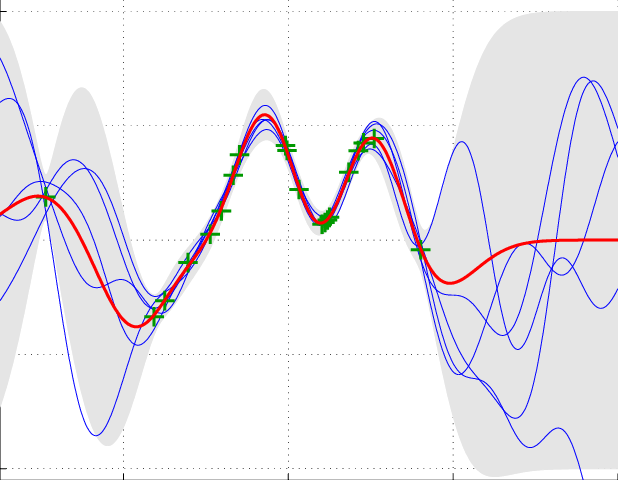
\includegraphics[width=0.4\textwidth]{pictures/files/final/gaussianprocess.png}%
    \caption{\textbf{Mean and variance of a Gaussian process's prediction}. Image from \cite{perez2013gaussian}. Intuitively, variance grows when samples are distant from training samples.}
    \label{fig:gp}%
\end{figure}%

\subsubsection{Discussion of the same norm and low similarity \Cref{ass:inter_sample} on source dataset}
\label{app:discussion_inter_sample}
\Cref{lemma:var_gp} shows that the variance only depends on the input distributions $p(X)$ without involving the label distributions $p(Y|X)$.
This formula highlights that the variance is related to shifts in input similarities (measured by $K$) between $X_{d_S}$ and $X_{d_T}$.
Yet, a more refined analysis of the variance requires additional assumptions, in particular to obtain a closed-form expression of $K(X_{d_S}, X_{d_S})^{-1}$.
\Cref{ass:inter_sample} is useful because then $K(X_{d_S}, X_{d_S})$ is diagonally dominant and can be approximately inverted (see \Cref{app:proof_ood_var}).

The first part of \Cref{ass:inter_sample} assumes that $\exists \lambda_S$ such that all training inputs $x_S\in X_{d_S}$ verify $K(x_S, x_S)= \lambda_S$.
Note that this equality is standard in some kernel machine algorithms \cite{ah2010normalized,ghojogh2021reproducing,rennie2005} and is usually achieved by replacing $K(x,x^\prime)$ by $\lambda_S \frac{K(x,x^\prime)}{\sqrt{K(x,x)}\sqrt{K(x^\prime,x^\prime)}}, \forall(x,x^\prime)\in {(X_{d_S}\cup X_{d_T})}^2$. 
In the NTK literature, this equality is achieved without changing the kernel by normalizing the samples of $X_{d_S}$ such that they lie on the hypersphere; this input preprocessing was used in \cite{Lee2018DeepNN}.
This is theoretically based: for example, the NTK $K(x, x^\prime)$ for an architecture with an initial fully connected layer only depends on $\|x\|,\|x^\prime\|,\langle x, x^\prime\rangle$ \cite{yang2019}. Thus in the case where all samples from $X_{d_S}$ are preprocessed to have the same norm, the value of $K(x_S,x_S)$ does not depend on $x_S\in X_{d_S}$; we denote $\lambda_S$ the corresponding value.

The second part of \Cref{ass:inter_sample} states that $\exists 0 \leq \epsilon \ll \lambda_S, \text{s.t.~} \forall x_S, x_S^\prime \in X_{d_S}^2, x_S\neq x_S^\prime \Rightarrow |K(x_S,x_S^\prime)|\leq\epsilon$, \ie that training samples are dissimilar and do not interact.
This diagonal structure of the NTK \cite{Jacot2018}, with diagonal values larger than non-diagonal ones, is consistent with empirical observations from \cite{seleznova2022neural} at initialization.
% at initialization, when the kernel regime is relaxed.
Theoretically, this is reasonable if $K$ is close to the RBF kernel $K_{h}\left(x, x^{\prime}\right)=\exp (-\left\|x-x^{\prime}\right\|_{2}^{2}/h)$ where $h$ would be the bandwidth: in this case, \Cref{ass:inter_sample} is satisfied when training inputs are distant in pixel space.

We now provide an analysis of the variance where the diagonal assumption is relaxed.
Specifically, we provide the sketch for proving an upper-bound of the variance when the NTK has a block-diagonal structure.
This is indeed closer to the empirical observations in \cite{seleznova2022neural} at the end of training, consistently with the local elasticity property of NNs \cite{He2020The}.
We then consider the dataset $d_{S^\prime} \subset d_S$ made of one sample per block, to which \Cref{ass:inter_sample} applies.
As decreasing the size of a training dataset empirically reduces variance \cite{brain1999effect}, the variance of $f$ trained on $d_S$ is upper-bounded by the variance of $f$ trained on $d_{S^\prime}$; the latter is given by applying \Cref{prop:var} to $d_{S^\prime}$.
We believe that the proper formulation of this idea is beyond the scope of this article and best left for future theoretical work.

\subsubsection{Expression of \ood variance}
\label{app:proof_ood_var}

\begin{proposition*}[\ref{prop:var}]
    Given $f$ trained on source dataset $d_S$ (of size $n_S$) with NTK $K$, under \Cref{ass:infinite_width,ass:inter_sample}, the variance on dataset $d_T$ is:%
    \begin{equation*} \tag{\ref{eq:int_var}}
        \mathbb{E}_{x_T\in X_{d_T}}[\varb(x_T)] = \frac{n_S}{2\lambda_S}\text{MMD}^{2}(X_{d_S}, X_{d_T}) + \lambda_T - \frac{n_S}{2\lambda_S}\beta_T + O(\epsilon),%
    \end{equation*}
    with $\text{MMD}$ the empirical Maximum Mean Discrepancy in the RKHS of $K^2(x,y)=(K(x,y))^2$;$\lambda_T \triangleq \mathbb{E}_{x_T \in X_{d_T}} K\left(x_T, x_T\right)$ and $\beta_T \triangleq \mathbb{E}_{(x_T,x_T^\prime)\in X_{d_T}^2, x_T \neq x_T^\prime} K^2\left(x_T, x_T^{\prime}\right)$ the empirical mean similarities resp. measured between identical (\wrt $K$) and different (\wrt $K^2$) samples averaged over $X_{d_T}$.%
\end{proposition*}
\begin{proof}
Our proof is original and is based on the posterior form of GPs in \Cref{lemma:var_gp}.
Given $d_S$, we recall \Cref{eq:var} that states $\forall x\in\X$:
\begin{align*}
    %\bar{\mu}(x) &=K(x, X_{d_S})\left(K_{X_{d_S}, X_{d_S}}+\sigma_{\epsilon}^{2} \mathbb{I}_{n}\right)^{-1} \boldsymbol{y} \\
    \varb(x) =K(x, x)-K(x, X_{d_S})K(X_{d_S}, X_{d_S})^{-1} K(x, X_{d_S})^\intercal.
\end{align*}
Denoting $B=K(X_{d_S},X_{d_S})^{-1}$ with symmetric coefficients $b_{i,j}=b_{j,i}$, then
\begin{equation} \label{eq:inversion}
    \varb(x) = K(x, x)-\sum_{\substack{1 \leq i \leq n_S \\ 1 \leq j \leq n_S}} b_{i, j} K(x, x_S^i) K(x, x_S^j).
\end{equation}

\Cref{ass:inter_sample} states that
$K(X_{d_S}, X_{d_S})=A+H$ where $A=\lambda_S\mathbb{I}_{n_S}$ and $H=(h_{ij})_{\substack{1 \leq i \leq n_S \\ 1 \leq j \leq n_S}}$ with $h_{i,i}=0$ and $\max_{i,j}|h_{i,j}|\leq\epsilon$.

We fix $x_T \in X_{d_T}$ and determine the form of $B^{-1}$ in two cases: $\epsilon=0$ and $\epsilon\neq 0$.

\paragraph{Case when $\epsilon=0$}
We first derive a simplified result, when $\epsilon=0$.

Then, $b_{i,i}=\frac{1}{\lambda_S}$ and $b_{i,j}=0$ \sut
$$
    \varb(x_T)=K(x_T, x_T)-\sum_{x_S\in X_{d_S}} \frac{K(x_T, x_S)^2}{\lambda_S}=K(x,x) - \frac{n_S}{\lambda_S} \mathbb{E}_{x_S\in X_{d_S}}[K^2(x, x_S)]
$$
We can then write:
\begin{align*}
    &\mathbb{E}_{x_T\in X_{d_T}} [\varb(x_T)] = \mathbb{E}_{x_T\in X_{d_T}}[K(x_T, x_T)] - \frac{n_S}{\lambda_S} \mathbb{E}_{x_T\in X_{d_T}}[\mathbb{E}_{x_S\in X_{d_S}}[K^2(x_T, x_S)]] \\
    &\mathbb{E}_{x_T\in X_{d_T}} [\varb(x_T)] = \lambda_T - \frac{n_S}{\lambda_S} \mathbb{E}_{x_S\in X_{d_S}, x_T\in X_{d_T}}[K^2(x_T, x_S)]. \\
\end{align*}
We now relate the second term on the r.h.s. to a MMD distance.
As $K$ is a kernel, $K^2$ is a kernel and its MMD between $X_{d_S}$ and $X_{d_T}$ is per \cite{Gretton2012}:
\begin{align*}
    %\text{MMD}^{2}(X_{d_S}, X_{d_T})=& \frac{1}{n_S(n_S-1)} \sum_{i=1}^{n_S} \sum_{j \neq i}^{n_S} K^2\left({x_S}_{i}, {x_S}_{j}\right)+\frac{1}{n_T(n_T-1)} \sum_{i=1}^{n_T} \sum_{j \neq i}^{n_T} K^2\left({x_T}_{i}, {x_T}_{j}\right) \\ &-\frac{2}{n_S n_T} \sum_{i=1}^{n_S} \sum_{j=1}^{n_T} K^2\left({x_S}_{i}, {x_T}_{j}\right) \\
    \text{MMD}^{2}(X_{d_S}, X_{d_T})= & \mathbb{E}_{x_S \neq x_S^\prime \in X_{d_S}^2}[K^2(x_S, x_S^\prime)]+\mathbb{E}_{x_T \neq x_T^\prime \in X_{d_T}^2}[K^2(x_T, x_T^\prime)]\\
    & \quad -2\mathbb{E}_{x_S\in X_{d_S}, x_T\in X_{d_T}}[K^2(x_T, x_S)].
\end{align*}
Finally, because $\epsilon=0$, $\mathbb{E}_{x_S \neq x_S^\prime \in X_{d_S}^2} K^2\left(x_S, x_S^{\prime}\right)=0$ \sut
\begin{align*}
    \mathbb{E}_{x_T\in X_{d_T}}[\varb(x_T)] &=\frac{n_S}{2\lambda_S}\text{MMD}^{2}(X_{d_S}, X_{d_T}) + \lambda_T\\
    & \quad\quad\quad -\frac{n_S}{2\lambda_S}\Big(\mathbb{E}_{x_T \neq x_T^\prime \in X_{d_T}^2} K^2\left(x_T, x_T^{\prime}\right)+\mathbb{E}_{x_S \neq x_S^\prime \in X_{d_S}^2} K^2\left(x_S, x_S^{\prime}\right)\Big) \\
    &=\frac{n_S}{2\lambda_S}\text{MMD}^{2}(X_{d_S}, X_{d_T}) +\lambda_T-\frac{n_S}{2\lambda_S}\mathbb{E}_{x_T \neq x_T^\prime \in X_{d_T}^2} K^2\left(x_T, x_T^{\prime}\right)\\
    &= \frac{n_S}{2\lambda_S}\text{MMD}^{2}(X_{d_S}, X_{d_T}) + \lambda_T - \frac{n_S}{2\lambda_S}\beta_T.
\end{align*}

We recover the same expression with a $O(\epsilon)$ in the general setting where $\epsilon\neq 0$.

%DO NOT DELETE
% old version with diagonal error
% \begin{align*}
%     \mathbb{E}_{x\in d_T}[\varb(x)] &=\frac{n_S}{2\lambda}\text{MMD}^{2}(X_{d_S}, X_{d_T}) + \lambda-\frac{n_S}{2\lambda}\Big(\mathbb{E}_{d_T} K^2\left(x_T, x_T^{\prime}\right)+\mathbb{E}_{d_S} K^2\left(x_S, x_S^{\prime}\right)\Big) \\
%     &=\frac{n_S}{2\lambda}\text{MMD}^{2}(X_{d_S}, X_{d_T}) +\lambda-\frac{n_S}{2\lambda}\mathbb{E}_{d_T} K^2\left(x_T, x_T^{\prime}\right)-\frac{n_S}{2\lambda}\mathbb{E}_{d_S} K^2\left(x_S, x_S^{\prime}\right) \\
%     &= \frac{n_S}{2\lambda}\text{MMD}^{2}(X_{d_S}, X_{d_T}) + \lambda - \frac{n_S}{2\lambda}\beta_T-\frac{n_S}{2\lambda} \frac{\lambda^2 n_S}{n_S^2} \\
%     &= \frac{n_S}{2\lambda}\text{MMD}^{2}(X_{d_S}, X_{d_T}) + \lambda - \frac{n_S}{2\lambda}\beta_T-\frac{n_S}{2\lambda} \frac{\lambda^2}{n_S}\\
%     &= \frac{n_S}{2\lambda}\text{MMD}^{2}(X_{d_S}, X_{d_T}) + \lambda - \frac{n_S}{2\lambda}\beta_T-\frac{\lambda}{2}\\
%     &= \frac{n_S}{2\lambda}\text{MMD}^{2}(X_{d_S}, X_{d_T}) + (\frac{\lambda}{2} - \frac{n_S}{2\lambda}\beta_T)
% \end{align*}
% We recover the same expression with a $O(\epsilon)$ in the general setting where $\epsilon\neq 0$.

%DO NOT DELETE
% \paragraph{Case when $\epsilon\neq0$}
% Now, we assume that $\epsilon \neq 0$.
% \Cref{ass:inter_sample} states that
% $$
%     K(X_{d_S}, X_{d_S}) = A + b c^\intercal \text{~where~} A=(1-\epsilon) \mathbb{I}_{n_S}, b=c\triangleq[\sqrt{\epsilon}, \cdots, \sqrt{\epsilon}]^\intercal \in \mathbb{R}^{n_S}
% $$

% We apply Sherman-Morrison to perform inversion:
% \begin{align*}
%     \left(\mathbf{A}+\mathbf{b} \mathbf{c}^{T}\right)^{-1}&=\mathbf{A}^{-1}-\frac{\mathbf{A}^{-1} \mathbf{b} \mathbf{c}^{T} \mathbf{A}^{-1}}{1+\mathbf{c}^{T} \mathbf{A}^{-1} \mathbf{b}} \\
%     &= \frac{1}{1-\epsilon} \mathbb{I}_{n_S}- \frac{1}{1+\frac{\epsilon}{1-\epsilon}n_S}\frac{\epsilon}{(1-\epsilon)}\mathbf{1}_{n_S} \\
%     &=\frac{1}{1-\epsilon} \mathbb{I}_{n_S}- \frac{\epsilon}{1+\epsilon (n_S-1)}\mathbf{1}_{n_S} \\
%     &= (\frac{1}{1-\epsilon}-\frac{\epsilon}{1-\epsilon + \epsilon n_S})\mathbb{I}_{n_S}- \frac{\epsilon}{1-\epsilon + \epsilon n_S}(\mathbf{1}_{n_S}-\mathbb{I}_{n_S})
% \end{align*}
% Therefore, \Cref{eq:inversion} can be developed using $b_{i,i}=\frac{1}{1-\epsilon}-\frac{\epsilon}{1-\epsilon + \epsilon n_S}$ and $b_{i,j}=- \frac{\epsilon}{1-\epsilon + \epsilon n_S}=O(\epsilon)$ and denoting $\frac{1}{\kappa_{\lambda_S,\epsilon}}=b_{i,i}> 0$ into:
% \begin{align*}
%     \varb(x)&=K(x, x)-\sum_{x_S\in X_{d_S}} \frac{K(x, x_S)^2}{\kappa_{\lambda_S,\epsilon}} + O(\epsilon) \\
%     \mathbb{E}_{d_S} [\varb(x)]&= K(x,x)-\mathbb{E}_{d_S}[ \frac{1}{\kappa_{\lambda_S,\epsilon}} \sum_{x_S\in X_{d_S}} K(x, x_S)^2] + O(\epsilon) \\
%     &= K(x,x)-\frac{1}{\kappa_{\lambda_S,\epsilon}}\mathbb{E}_{x_S\sim p_S(X)}[K(x, x_S)^2] + O(\epsilon)
% \end{align*}
% As for the case $\epsilon=0$, we obtain:
% \begin{align*}
%     &\mathbb{E}_{x\in d_T}[\varb(x)] \\
%     &=\frac{1}{2\kappa_{\lambda_S,\epsilon}}\text{MMD}^{2}(X_{d_S}, X_{d_T}) + \mathbb{E}_{x_T\in X_{d_T}} K(x_T, x_T) -\frac{1}{2\kappa_{\lambda_S,\epsilon}}\Big(\mathbb{E}_{p_T(X)} K^2\left(x_T, x_T^{\prime}\right)+\mathbb{E}_{x_S\in X_{d_S}} K^2\left(x_S, x_S^{\prime}\right)\Big) + O(\epsilon)\\
%     &=\frac{1}{2\kappa_{\lambda_S,\epsilon}}\text{MMD}^{2}(X_{d_S}, X_{d_T}) + 1-\frac{1}{2\kappa_{\lambda_S,\epsilon}} 2 {\lambda}^2 + O(\epsilon) \\
%     &= \frac{1}{2\kappa_{\lambda_S,\epsilon}}\text{MMD}^{2}(X_{d_S}, X_{d_T}) + (1-\frac{1^2}{\kappa_{\lambda_S,\epsilon}}) + O(\epsilon)
% \end{align*}
% Moreover, as $\frac{1}{\kappa_{\lambda_S,\epsilon}}=\frac{1}{1-\epsilon}-\frac{\epsilon}{1-\epsilon + \epsilon n_S}$,
% \begin{align*}
%     1-\frac{1^2}{\kappa_{\lambda_S,\epsilon}} = 1 - \frac{1^2}{1-\epsilon} + O(\epsilon) = -\frac{\epsilon1}{1-\epsilon} + O(\epsilon) = O(\epsilon)
% \end{align*}
% Therefore
% $$
%     \mathbb{E}_{x\in d_T}[\varb(x)] = \frac{1}{2\kappa_{\lambda_S,\epsilon}}\text{MMD}^{2}(X_{d_S}, X_{d_T}) + O(\epsilon)
% $$
% where $\frac{1}{\kappa_{\lambda_S,\epsilon}} \rightarrow 1$ when $\epsilon \rightarrow 0$.

\paragraph{Case when $\epsilon\neq 0$}
We denote
$I:\left\{\begin{array}{cl}\mathrm{GL}_{n_S}(\mathbb{R}) & \rightarrow \mathrm{GL}_{n_S}(\mathbb{R}) \\ A & \mapsto A^{-1}\end{array}\right.$
the inversion function defined on $\mathrm{GL}_{n_S}(\mathbb{R})$, the set of invertible matrices of $\mathcal{M}_{n_S}(\mathbb{R})$.

The function $I$ is differentiable \cite{magnus2019matrix} in all $A\in \mathrm{GL}_{n_S}(\mathbb{R})$ with its differentiate given by the linear application
$dI_A:\left\{\begin{array}{cl}\mathcal{M}_{n_S}(\mathbb{R})&\rightarrow \mathcal{M}_{n_S}(\mathbb{R}) \\ H &\mapsto - A^{-1}HA^{-1}\end{array}\right.$. Therefore, we can perform a Taylor expansion of $I$ at the first order at $A$:
\begin{align*}
    I(A+H)&=I(A)+dI_A(H)+o(\|H\|), \\
    (A+H)^{-1}&=A^{-1}-A^{-1}HA^{-1}+o(\|H\|).
\end{align*}
where $\|H\|\leq n_S\epsilon=O(\epsilon)$. Thus,
\begin{align*}
    (\lambda_S\mathbb{I}_{n_S}+H)^{-1}&=(\lambda_S\mathbb{I}_{n_S})^{-1}-(\lambda_S\mathbb{I}_{n_S})^{-1}H(\lambda_S\mathbb{I}_{n_S})^{-1}+O(\epsilon) =\frac{1}{\lambda_S}\mathbb{I}_{n_S}-\frac{1}{\lambda_S^2}H+O(\epsilon), \\
    \forall i \in \llbracket1, n_S\rrbracket, b_{ii}&=\frac{1}{\lambda_S}-\frac{1}{\lambda_S^2}h_{i,i}+o(\epsilon)=\frac{1}{\lambda_S}+O(\epsilon), \\
    \forall i \neq j \in \llbracket1, n_S\rrbracket, b_{ij}&=-\frac{1}{\lambda_S^2}h_{i,j}+o(\epsilon)=O(\epsilon).
\end{align*}

Therefore, when $\epsilon$ is small, \Cref{eq:inversion} can be developed into:
\begin{align*}
    \varb(x_T)&=K(x_T, x_T)-\sum_{x_S\in X_{d_S}} (\frac{1}{\lambda_S}+O(\epsilon)) K(x_T, x_S)^2 + O(\epsilon) \\
    &= K(x_T,x_T)- \frac{n_S}{\lambda_S} \mathbb{E}_{x_S\in X_{d_S}}[K(x_T, x_S)^2] + O(\epsilon)
\end{align*}
Following the derivation for the case $\epsilon=0$, and remarking that under \Cref{ass:inter_sample} we have $\mathbb{E}_{x_S \neq x_S^\prime \in X_{d_S}^2} K^2\left(x_S, x_S^{\prime}\right)=O(\epsilon^2)$, yields:
\begin{equation*}
    \mathbb{E}_{x_T\in X_{d_T}}[\varb(x_T)] = \frac{n_S}{2\lambda_S}\text{MMD}^{2}(X_{d_S}, X_{d_T}) + \lambda_T - \frac{n_S}{2\lambda_S}\beta_T+ O(\epsilon).
\end{equation*}

% When $\lambda=\frac{n_S}{2}$,
% $$
%     \mathbb{E}_{x\in d_T}[\varb(x)] = \text{MMD}^{2}(X_{d_S}, X_{d_T}) + (\frac{n_S}{4} - \beta_T)+ O(\epsilon)
% $$

% Finally, $\beta_T = \frac{\lambda^2 n_T + \alpha_T}{n_T^2}$ where $\alpha_T=\sum_{x_T \neq x_T^\prime} K^2(x_T, x_T^\prime)$ \sut
% $$
%  \frac{n_S}{4} - \beta_T = \frac{n_S}{4} - \frac{\frac{n_S^2}{4} n_T}{n_T^2} - \frac{\alpha_T}{n_T^2}= \frac{n_S}{4} - \frac{n_S^2}{4 n_T} - \frac{\alpha_T}{n_T^2} = \frac{n_S}{4}(1-\frac{n_S}{n_T})-\frac{\alpha_T}{n_T^2}
% $$
% denoting $\kappa_T=\frac{\alpha_T}{n_T^2}\geq 0$
% $$
%     \mathbb{E}_{x\in d_T}[\varb(x)] = \text{MMD}^{2}(X_{d_S}, X_{d_T}) - \frac{n_S}{4}(\frac{n_S}{n_T}-1) - \kappa_T + O(\epsilon)
% $$
\end{proof}

% \begin{lemma}\label{lemma:var_mmd0}
%     When $p_S=p_T$, $\mathbb{E}_{x_T\in X_{d_T}}[\varb(x_T)] = \lambda_T + O(\epsilon)$
% \end{lemma}
% \begin{proof}
%     When $p_S=p_T$, $\text{MMD}^{2}(X_{d_S}, X_{d_T})=0$. The $p_S=p_T$ condition also constrains that $T$ also verifies \Cref{ass:inter_sample} thus $\beta_T=O(\epsilon)$.
%     In conclusion, $\lambda_T$ is the only term left from \Cref{prop:var}.
% \end{proof}
% We recover that variance is small in \iid for infinitely large networks \cite{neal2018modern,belkin2019reconciling,pmlr-v119-d-ascoli20a}.
% \begin{proof}
%     \begin{align*}
%         \mathbb{E}_{x_T\in X_{d_T}} [\varb(x_T)] &= \frac{\lambda}{2} - \frac{n_S}{\lambda} \mathbb{E}_{x_S\in X_{d_S}, x_T\in X_{d_T}}[K^2(x_T, x_S)] + O(\epsilon)\\
%         &=\frac{n_S}{4} -2\mathbb{E}_{x_S\in X_{d_S}, x_T\in X_{d_T}}[K^2(x_T, x_S)]+O(\epsilon)
%     \end{align*}
%     \begin{align*}
%         \text{MMD}^{2}(X_{d_S}, X_{d_T}) &=\mathbb{E}_{X_{d_S}} K^2\left(x_S, x_S^{\prime}\right)+\mathbb{E}_{X_{d_T}} K^2\left(x_T, x_T^{\prime}\right)-2 \mathbb{E}_{X_{d_S}, X_{d_T}} K^2(x_S, x_T) \\
%         &= \frac{\lambda^2 n_S + O(\epsilon^2)}{n_S^2}  + \frac{\lambda^2 n_T}{n_T^2} + \kappa_T -2 \mathbb{E}_{X_{d_S}, X_{d_T}} K^2(x_S, x_T) \\
%         &= \frac{\lambda^2}{n_S}  + \frac{\lambda^2 n_T}{n_T^2} + \kappa_T -2 \mathbb{E}_{X_{d_S}, X_{d_T}} K^2(x_S, x_T) + O(\epsilon^2) \\
%         &= \frac{n_S}{4}  + \frac{n_S^2}{4n_T} + \kappa_T -2 \mathbb{E}_{X_{d_S}, X_{d_T}} K^2(x_S, x_T) + O(\epsilon^2)
%     \end{align*}
%     When $\text{MMD}^{2}(X_{d_S}, X_{d_T})=0$,
%     \begin{align*}
%         -\frac{n_S}{4} - \frac{n_S^2}{4n_T} - \kappa_T  + O(\epsilon^2) = -2 \mathbb{E}_{X_{d_S}, X_{d_T}} K^2(x_S, x_T)
%     \end{align*}
%     \begin{align*}
%         \mathbb{E}_{x_T\in X_{d_T}} [\varb(x_T)] &=  \frac{n_S}{4} -\frac{n_S}{4} - \frac{n_S^2}{4n_T} - \kappa_T  + O(\epsilon^2) \\
%         &= - \frac{n_S^2}{4n_T} - \kappa_T  + O(\epsilon^2)
%     \end{align*}
% \end{proof}

\subsubsection{Variance and initialization}
\label{remark:mmdk}

The MMD depends on the kernel $K$, \ie only on the initialization of $f$ in the kernel regime per \cite{Jacot2018}. Thus, to reduce variance, we could act on the initialization to match $p_S(X)$ and $p_T(X)$ in the RKHS of $K^2$.
This is consistent with \Cref{subsec:expression_ood_bias} that motivated matching the train and test in features.
In our paper, we used the standard pretraining from ImageNet \cite{krizhevsky2012imagenet}, as commonly done on DomainBed \cite{gulrajani2021in}.
The Linear Probing \cite{kumar2022finetuning} initialization of the classifier was shown in \cite{kumar2022finetuning} to prevent the distortion of the features along the training.
This could be improved by pretraining the encoder on a task with fewer domain-specific information, \eg CLIP \cite{radford2021learning} image-to-text translation as in \cite{ruan2022optimal}.